\begin{frame}
	\frametitle{Algoritmos de força bruta}
	\begin{figure}
		\centering
		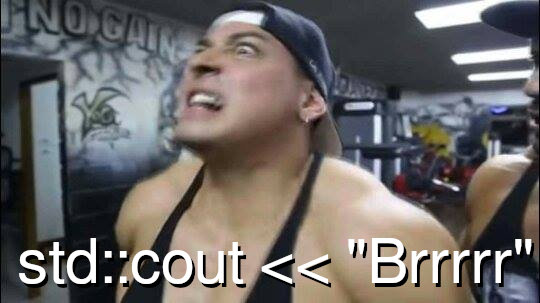
\includegraphics[width=.9\linewidth]{images/bodyBuildPorra}
		\caption{Processei pra crl! Vai dar sim!}
		\label{fig:bodybuildporra}
	\end{figure}
	
\end{frame}

\begin{frame}
	\frametitle{Algoritmos de força bruta}
	\par São aqueles cuja a definição não se pode expressar em termos polinomiais ou cujos tempos são muito grandes, geralmente são feitos para mapear todas as opções dentro de um certo espaço de procura resultando assim em ordens de tempo muito grandes.
	
	\par Geralmente tais algoritmos estão ligados a um pensamento mais direto de resolução do problema e dependente do poder de processamento do computador e não da inteligência na modelagem.\newline
	
	\par Alguns dos exemplos que já vimos são o \textbf{burbble-Sort}, \textbf{Selection-Sort}, além de outros como \textbf{Busca sequencial}, \textbf{multiplicação de matrizes}, etc.\newline
	
	\par No entanto, existem técnicas como o \textbf{bactracking} ou \textbf{retro-rastreamento} e \textbf{branching-and-bound} ou \textbf{ramificar e limitar} que são estratégias que usam uma \textbf{árvores de estados} e podem melhorar um pouco tais tempos de execução.	
\end{frame}

\begin{frame}
	\frametitle{Algoritmos de busca em grafos}
	\framesubtitle{Árvore de estados}
	\par Esta árvore indica em cada um dos seus nós um estado alcançado pelo sistema, assim, é possível, considerando-se certas condições, julgar a possibilidade ou a utilidade de se fazer novos testes, ou ainda, se é necessário voltar a algum estado anterior. Existem técnicas como o \textbf{backtracking} ou \textbf{retro-rastreamento} e \textbf{branching-and-bound} ou \textbf{ramificar e limitar} que são estratégias que usam uma \textbf{árvores de estados} e podem melhorar um pouco os tempos de execução de algoritmos de força bruta.
	
	\tikzset{
		tree/.style={
			every node/.style={rectangle,draw},
			level 1/.style={sibling distance=60mm},
			level 2/.style={sibling distance=30mm},
			level 3/.style={sibling distance=20mm},
		},
		fontbf/.style={font=\bfseries}
	}
	
	\begin{figure}
		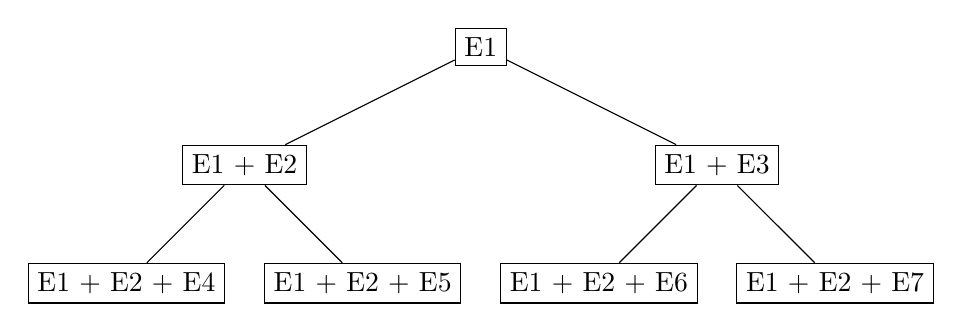
\begin{tikzpicture}[tree]
			\node {E1}
			child{
				node{E1 + E2}
				child{node{E1 + E2 + E4}}
				child{node{E1 + E2 + E5}}
			}
			child{
				node{E1 + E3}
				child{node{E1 + E2 + E6}}
				child{node{E1 + E2 + E7}}
			};
		\end{tikzpicture}
	\end{figure}
\end{frame}

\begin{frame}
	\frametitle{Algoritmos de força bruta}
	\framesubtitle{Retro-rastreamento - Ramificar e limitar}
	\par Dado um problema de otimização, se o custo de uma solução possível ultrapassou o valor de outra então se pode parar como o processamento daquela possibilidade.
		\begin{columns}
		\begin{column}{0.5\textwidth}
			\begin{figure}
				\centering
				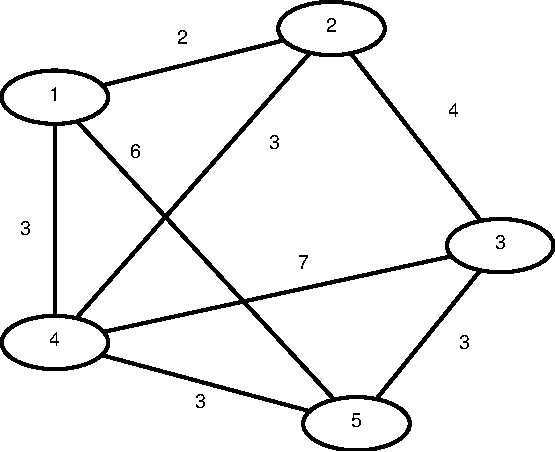
\includegraphics[width=0.8\linewidth]{images/grafoForcaBruta}
				\caption{Caixeiro viajante}
				\label{fig:grafoforcabruta}
			\end{figure}
		\end{column}
		\begin{column}{0.5\textwidth}
			\begin{figure}
				\centering
				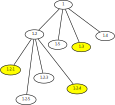
\includegraphics[width=0.8\linewidth]{images/arvoreEstadoForcaBruta}
				\caption{Árvore de estados}
				\label{fig:arvoreestadoforcabruta}
			\end{figure}
		\end{column}
	\end{columns}
\end{frame}

\begin{frame}
	\frametitle{Algoritmos de força bruta}
	\framesubtitle{Retro-rastreamento - Ramificar e limitar - Exercício}
	\par Posicione 4 rainhas em um tabuleiro 4x4 sem que elas se ataquem. Monte a árvore de estados com Retro-rastreamento e Ramificar e limitar.
\end{frame}